\documentclass[11pt]{scrartcl}

\usepackage[utf8]{inputenc} % Input encoding
\usepackage[T1]{fontenc} % Font encoding
\usepackage{siunitx} % Provides the \SI{}{} and \si{} command for typesetting SI units
\usepackage{graphicx} % Required for the inclusion of images
\usepackage{natbib} % Required to change bibliography style to APA
\usepackage{amsmath} % Required for some math elements 
\usepackage{lmodern} % Font used in the document
\usepackage{hyperref} % To add link in the document
\usepackage[headsepline]{scrpage2} % For headers and footers with KOMA classes
\usepackage{todonotes}
\usepackage{tikz, pgfplots}
\usepackage{pgfplotstable}
\usepackage{booktabs}
\usepackage{array}
\usepackage{colortbl}
\usepackage{enumitem} % Enumeration package
\usepackage[english]{babel} 

\synctex=1 % For syncing skim with Emacs

\setlength\parindent{0pt} % Removes all indentation from paragraphs

\renewcommand{\labelitemi}{\textbullet} % make items in itemize environment bullets rather that dashes
\renewcommand{\labelenumi}{\alph{enumi}.} % Make numbering in the enumerate environment by letter rather than
                                % number (e.g. section 6)

%\usepackage{times} % Uncomment to use the Times New Roman font

\usepackage{listings}
\usepackage[framed,autolinebreaks,useliterate]{mcode}

% Pgf cycle colors
\pgfplotsset{cycle list name = exotic, compat=1.12}


%----------------------------------------------------------------------------------------
%	DOCUMENT INFORMATION
%----------------------------------------------------------------------------------------

\addtokomafont{disposition}{\normalfont\bfseries} % Make title/sections/subsections font the same as the rest
                                % of the document

\title{Philip Morris: Data Analysis Improvement of Ciliary Beating of 3D Epithelial Tissue\\\vspace{1cm}Final report\vspace{1cm}} % Title

\author{Simon Jenni \& Laurent Hayez} % Author name

\date{\today} % Date for the report

\begin{document}

%----------------------------------------------------------------------------------------
%	HEADERS AND FOOTERS
%----------------------------------------------------------------------------------------

\setfootsepline[text]{.4pt}

\pagestyle{scrheadings}
\automark[section]{section}
\ihead{{\sc Data Analysis Improvement of Ciliary Beating of 3D Epithelial Tissue}}
\ohead{}
\chead{}
\ifoot[Final report]{{\sc Final report}}
\ofoot[\pagemark]{\pagemark}
\cfoot[]{}

\maketitle % Insert the title, author and date

\thispagestyle{empty}

\begin{center}
\begin{tabular}{l r !{\textendash} l}
Contact: & Simon Jenni & \href{mailto:simujenni@students.unibe.ch}{simujenni@students.unibe.ch} \\ % Partner names
& Laurent Hayez: & \href{mailto:laurent.hayez@unine.ch}{laurent.hayez@unine.ch}\\
Supervisor: & Patrice Leroy: & \href{mailto:Patrice.Leroy@pmi.com)}{Patrice.Leroy@pmi.com} % Instructor/supervisor
\end{tabular}
\end{center}

% If you wish to include an abstract, uncomment the lines below
% \begin{abstract}
% Abstract text
% \end{abstract}

\vspace{1cm}
\renewcommand{\contentsname}{Table of contents}
\tableofcontents



%----------------------------------------------------------------------------------------
%	SECTION 1
%----------------------------------------------------------------------------------------

\section{Project Description}

\subsection{Project Context}

Philip Morris International (PMI) is a global cigarette and tobacco company with headquarters in Lausanne. The
research and development program of PMI focuses on the development of products with the potential to reduce
the risk of tobacco related diseases. To this end, new products are tested against ordinary cigarettes by
exposing human tissue cultures to smoke or aerosol of both products. The effect of the exposure is then
analysed by observing different features of the tissue, one of which is the ciliary beating.


\subsection{Goals and Objectives of the Project}

The goal of this project is to implement a tool for the automatic analysis of ciliary beating in tissue
movies. Concretely the objectives are the following:
\begin{itemize}
\item Allowing batch processing of video-data contained in a folder (including subfolders). 
\item Pre-processing of the video data in order to remove noise by smoothing with a customisable 3D kernel.
\item Scoring the tissue surface activity using simple descriptive statistics and storing the results in an
  activity image.
\item Determining the frequency distribution given per region of interest (ROI) and extracting the
  dominant frequency.
\item Processing should be possible on multiple scales, i.e. ROI of variable size. 
\item Illustrating the phase of the beating frequency.
\end{itemize}

Part of the project is also an evaluation of the performance of different techniques applied to the
problem and other research objectives such as:

\begin{itemize}
\item Evaluating the effect of the ROI size on performance.
\item Evaluating the probable shape of the beating pattern on a by beating movie basis.
\item Comparing different techniques for the frequency analysis (e.g. FFT and wavelet transform).
\end{itemize}

Given the scope of this project and the relatively large amount of objectives, it should be noted that some of
the objectives have been given a higher priority than others. The ultimate goal of this project is to provide
a tool for frequency analysis and task-priorities were therefore weighted with this goal in mind. This
means for example that de-noising, a whole subject on it's own, has not be studied and evaluated as
extensively as techniques for frequency analysis.

 
%----------------------------------------------------------------------------------------
%	SECTION 2
%----------------------------------------------------------------------------------------

\section{Methodology}

The implementation of the tool was carried out in Matlab. The decision to use Matlab has been taken in
agreement with the client and is based on the ease of handling image and video processing and the relatively
fast development time that Matlab provides.  Git has been used as version control tool.

Development has been done in an incremental and iterative fashion roughly following the SCRUM framework. The
objectives have been distributed across sprints of two weeks each. To keep track
of the progress and help manage the project we have been using Taiga, an open source project management
platform similar to JIRA. Both the client and project stakeholders were given access to Taiga and have been able
to follow the progress.

Testing of our implementation using synthetic test-data has been an integral part of
the development process to ensure correctness of the implementation. In order to maintain a high code-quality, code reviews by the other respective
developer have been performed for every task.

\subsection{State of the art}

The arguably most accurate method for analysing the ciliary beating frequency is the direct measurement from
high-speed video recordings. This is of course very time-consuming and therefore several automated methods
have been proposed. The most commonly used approaches for the automated analysis of ciliary beating are based
on using the Fast Fourier Transform (FFT) to analyse intensity-signals in a region of interest and has been the
principal approach and starting point for further exploration used in this project. Other methods such as
photomultiplier and modified photodiode techniques rely on different hardware and inputs and are therefore not
considered.

%----------------------------------------------------------------------------------------
%	SECTION 3
%----------------------------------------------------------------------------------------

\section{Realisation} 

\subsection{Frequency Analysis}

\begin{minipage}{\linewidth}
  \begin{lstlisting}[caption={Function performing the frequency analysis using the FFT.}, label=list:res]
function [ power, f, domFreqs, domPhase ] = performFFT( data, fs )
%PERFORMFFT performs frequency analysis using the fast fourier transform
% Input:
%   data - 3D array of extracted video data (width x height x frames)
%   fs - Sampling frequency of the input data
% Output:
%   power - Power of resulting discrete fourier transform
%   f - Frequency range
%   domFreqs - Dominant frequency per region of interest 
%   domPhase - Phase corresponding to dominant frequency
% See also BATCHANALYSEFOLDER, WTANALYSIS.
  \end{lstlisting}
\end{minipage}



\subsection{Activity Analysis}

\begin{minipage}{\linewidth}
  \begin{lstlisting}[caption={Function performing the activity analysis using entropy.}, label=list:res]
function entropy = computeEntropy(data) 
%COMPUTEENTROPY Computes pixel-wise entropy of the provided video-data.
% Input:
%   data - 3D array of extracted video data (width x height x frames)
% Output:
%   entropy - 2D array of size (width x height) where entropy(i,j) is the
%             entropy along data(i,j,:)
% See also PLOTRESULTS, ACTIVITYFROMPOWER.
  \end{lstlisting}
\end{minipage}

\subsection{Smoothing for Noise-Removal}

\begin{minipage}{\linewidth}
  \begin{lstlisting}[caption={Function performing the noise removal.}, label=list:res]
function [ data ] = filter3d( data, dims, sigmas, type )
%FILTER3D Filters the provided 3D-array data with a 3D-gaussian kernel with
%dimensions specified in dims and gaussians with standard-deviations
%specified by sigmas. Filtering in 'time' can optionally be performed using
%median-filtering.
% Input:
%   data - 3D array (width x height x frames)
%   dims - Vector (hx, hy, hz) of filter dimensions
%   sigmas - Vector (sx, sy, sz) parameters for gaussian filters
%   type - 'gaussian' or 'median' defining type of 3rd dimension filter
% Output:
%   data - filtered input
% See also BATCHANALYSEFOLDER.
  \end{lstlisting}
\end{minipage}

\subsection{Extracting Probable Beating Pattern}

\begin{minipage}{\linewidth}
  \begin{lstlisting}[caption={Function for extracting the probable beating pattern.}, label=list:res]
function [ shape ] = probableShapeFromData( dominantFreqs, phase, data,...
    activity, fs )
%PROBABLESHAPEFROMDATA Computes the probable shape of the beating pattern 
%from the results of the FFT and the underlying data.
%Note: The FFT should be computed using ROI-size=1 for use with this 
%function.
% Input:
%   dominantFreqs - 2D array of size (w x h) with dominant frequencies per 
%                   pixel 
%   phase - 2D array of corresponding phases per pixel
%   data - 3D array of extracted video data of size (w x h x t)
%   activity - 2D array of activities phases per pixel
%   fs - Sampling frequency of the input data
% Output:
%   shape - Curve fitted to the data using smoothing-splines
% See also PERFORMFFT, COMPUTEENTROPY, ACTIVITYFROMPOWER.  
\end{lstlisting}
\end{minipage}


\subsection{Batch Processing of the Data}

\begin{minipage}{\linewidth}
  \begin{lstlisting}[caption={Function for extracting data from videos.}, label=list:res]
function batchExtractFolder( extractFolder, storeFolder, reload )
%BATCHEXTRACTFOLDER Extracts data of all the videos in the folder 
%extractFolder (including subfolders) and saves it to storeFolder for later 
%analysis. Note that if reload is set to false and the video has already 
%been extracted, the video will not be extracted again.
% Input:
%   folderPath - String indicating the path of the video-data
%   storeFolder - Folder where the extracted data should be stored
%   reload - Boolean value (already extracted videos skipped if false)
% See also EXTRACTVIDEODATA, SAVEEXTRACTEDDATA and ALREADYEXTRACTED.
\end{lstlisting}
\end{minipage}

\begin{minipage}{\linewidth}
  \begin{lstlisting}[caption={Function for analysing extracted data.}, label=list:res]
function batchAnalyseFolder( folderPath, fs, roiSize, resultsDir,...
    preProcess, method, waveletType )
%BATCHANALYSEFOLDER Anlayses all files in the given folder using the
%specified parameters and saves the results to the folder resultsDir.
% Input:
%   folderPath - Path to folder of exctracted video files to be analysed
%   fs - Sampling frequency of the data to be analysed
%   roiSize - Integer or vector [sx, sy] specifying the ROI-size
%   resultsDir - Path to directory where results should be stored
%   preProcess - Function handle for pre-processing function of extracted
%                data (e.g. denoising)
%   method - String indicating which method to use for analysis ("wt",
%            "fft" or "both")
%   waveletType - Specifies which wavelet to use for the wavelet transform.
%                 'morl' is used by default
% See also BATCHEXTRACTFOLDER, FILTER3D.
\end{lstlisting}
\end{minipage}


\subsection{GUI}


%----------------------------------------------------------------------------------------
%	SECTION 4
%----------------------------------------------------------------------------------------

\section{Results}

\subsection{Effect of ROI size on performance}
\label{sec:effect-roi-size}

We measured the computational time of the FFT analysis and the WT analysis for different ROI sizes on the
initial cylia beating movie. The ROI sizes tested were $1$, $[3, 4]$ and $[6, 8]$. The results are plotted in
Figure \ref{fig:computational-time}.

\pgfplotstableread{speed_results.dat}\speed
\begin{figure}[ht]
  \begin{minipage}{0.4\linewidth}
    \centering
    \pgfplotstableset{%
      fixed zerofill,
      precision=3,
      every head row/.style={before row=\toprule,after row=\midrule},
      every last row/.style={after row=\bottomrule}
    }
    \pgfplotstabletypeset[columns={FFT,WT}]\speed
    
  \end{minipage}
  \begin{minipage}{0.6\linewidth}
    \centering
    \begin{tikzpicture}[scale=1]
      \begin{axis}[
        scaled ticks=base 10:0,
        xlabel = {ROI sizes},
        ylabel = {Time (s)},
        title={Computational time of the FFT and WT},
        xtick = {1,2,3},
        xticklabels={{ROI $1$}, {ROI $[3, 4]$}, {ROI $[6, 8]$}},
        xticklabel style={rotate=45,anchor=east, scale=0.9}
        ]
        \addplot table[y = FFT] from \speed ; 
        \addlegendentry{FFT} ;
        \addplot table[y = WT] from \speed ;
        \addlegendentry{WT} ;    
      \end{axis}
    \end{tikzpicture}
  \end{minipage}
  \caption{Computational time of the FFT and WT for different ROI sizes}
  \label{fig:computational-time}
\end{figure}

Interestingly, computing the FFT pixel wise takes approximately 2 minutes and 40 seconds, while it takes 25
minutes for the WT. However, as soon as we increase the ROI size, the computational time for the WT decreases
drastically. It should be noted that the computations were run with \texttt{batchAnalyseFolder}, hence the
times presented here are greater than if we had only used \texttt{performFFT} and \texttt{WTAnalysis} instead.

\subsection{Effects of wavelet types}
\label{sec:effects-wavel-types}

The code currently supports only two types of wavelet types (two of the functions used support almost
exclusively distinct wavelet types):
\begin{itemize}
\item \texttt{morl} (Morlet wavelets),

\item \texttt{mexh} (Mexican hat wavelets).
\end{itemize}

However, there are significant differences between the results we obtain with these two wavelets. You can
compare Figure \ref{fig:morl} with Figure \ref{fig:mexh}. Although the spectrums are similar, the results we obtain with the Morlet wavelet are much
closer to the results we obtain with the fast Fourier transform.

\begin{figure}[h]
  \centering
  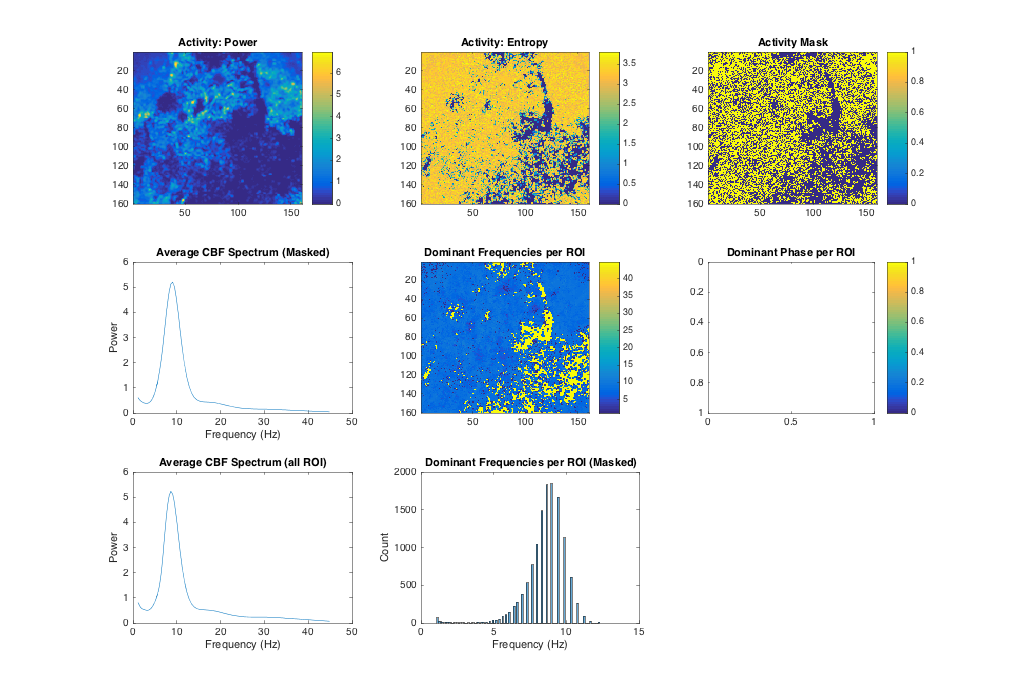
\includegraphics[scale=0.5]{Cylia_beating_movie_mat_Results.png}
  \caption{Results with \texttt{morl} wavelets}
  \label{fig:morl}
\end{figure}

\begin{figure}[h]
  \centering
  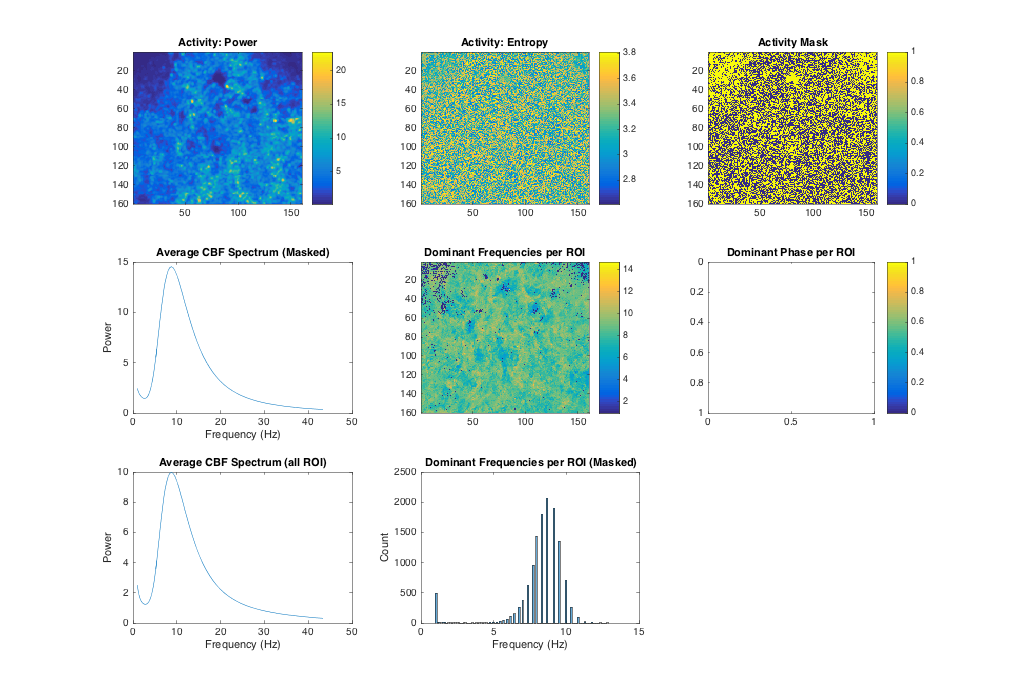
\includegraphics[scale=0.5]{Cylia_beating_movie_mexh_mat_Results.png}
  \caption{Results with \texttt{mexh} wavelets}
  \label{fig:mexh}
\end{figure}

\subsection{Comparison of the techniques used}
\label{sec:comp-techn-used}


%----------------------------------------------------------------------------------------
%	SECTION 6
%----------------------------------------------------------------------------------------

\section{Recommendations}


\subsection{Statement of Recommendations}


\subsection{Limitations}


\subsection{Outstanding Issues and Perspective for Future Work}



%----------------------------------------------------------------------------------------
%	SECTION 7
%----------------------------------------------------------------------------------------

\section{[Other relevant section]}








%----------------------------------------------------------------------------------------


\end{document}